\documentclass[journal]{IEEEtran}
\usepackage[a5paper, margin=10mm, onecolumn]{geometry}
\usepackage{lmodern}

\setlength{\headheight}{1cm}
\setlength{\headsep}{0mm}

\usepackage{gvv-book}
\usepackage{gvv}
\usepackage{cite}
\usepackage{amsmath,amssymb,amsfonts,amsthm}
\usepackage{graphicx}
\graphicspath{{./figs/}}
\usepackage{xcolor}
\usepackage{txfonts}
\usepackage{enumitem}
\usepackage{mathtools}
\usepackage{hyperref}
\usepackage{tikz}
\usepackage{tkz-euclide}

\begin{document}

\bibliographystyle{IEEEtran}
\vspace{3cm}

\title{4.11.14}
\author{EE25BTECH11036 - M Chanakya Srinivas}
\maketitle

\renewcommand{\thetable}{\theenumi}
\setlength{\intextsep}{10pt}
\renewcommand\theequation{\arabic{equation}}

\section*{Question}
Find the value of \(\lambda\) for which the following lines are perpendicular to each other. Hence determine whether the lines intersect or not.
\begin{align}
\frac{x-5}{5\lambda+2} &= \frac{2-y}{5} = \frac{1-z}{-1}, \label{eq:l1}\\
\frac{x}{1} &= \frac{y+\tfrac{1}{2}}{2\lambda} = \frac{z-1}{3}. \label{eq:l2}
\end{align}


\section*{Solution}

From the symmetric form, the point and direction vectors of each line are
\begin{align}
\vec{A} &= \myvec{5\\[2pt]2\\[2pt]1}, &
\vec{m_1} &= \myvec{5\lambda+2\\[2pt]-5\\[2pt]1}, \label{eq:a_m1}\\
\vec{B} &= \myvec{0\\[2pt]-\tfrac{1}{2}\\[2pt]1}, &
\vec{m_2} &= \myvec{1\\[2pt]2\lambda\\[2pt]3}. \label{eq:b_m2}
\end{align}

\noindent\textbf{Perpendicular condition:}
\begin{align}
\vec{m_1}^\top \vec{m_2} &= 0, \notag\\
(5\lambda+2)(1) + (-5)(2\lambda) + (1)(3) &= 0, \notag\\
5\lambda + 2 - 10\lambda + 3 &= 0, \notag\\
-5\lambda + 5 &= 0, \notag\\
\Rightarrow \boxed{\lambda = 1}. \label{eq:lambda}
\end{align}

Substituting $\lambda=1$,
\begin{align}
\vec{m_1} = \myvec{7\\[2pt]-5\\[2pt]1}, \quad 
\vec{m_2} = \myvec{1\\[2pt]2\\[2pt]3}. \label{eq:m1m2}
\end{align}

The matrix $M$ and vector $\vec{B}-\vec{A}$ are
\begin{align}
M = \myvec{7 & 1\\[2pt]-5 & 2\\[2pt]1 & 3}, \quad 
\vec{B}-\vec{A} = \myvec{-5\\[2pt]-\tfrac{5}{2}\\[2pt]0}. \label{eq:M_BA}
\end{align}

\noindent The lines intersect if
\begin{align}
\text{rank}\myvec{M & \vec{B}-\vec{A}} = 2. \label{eq:intersect}
\end{align}

\section*{RREF Calculation}

Form the augmented matrix:
\begin{align}
\myvec{
7 & 1 & -5\\
-5 & 2 & -\tfrac{5}{2}\\
1 & 3 & 0
}
\end{align}

\noindent Perform row operations:

\begin{align}
R_2 &\leftarrow R_2 + \tfrac{5}{7}R_1 = 
\myvec{7 & 1 & -5\\[4pt]0 & \tfrac{19}{7} & -\tfrac{75}{14}\\[4pt]1 & 3 & 0}, \\
R_3 &\leftarrow R_3 - \tfrac{1}{7}R_1 = 
\myvec{7 & 1 & -5\\[4pt]0 & \tfrac{19}{7} & -\tfrac{75}{14}\\[4pt]0 & \tfrac{20}{7} & \tfrac{5}{7}}. 
\end{align}

Next,
\begin{align}
R_2 &\leftarrow \tfrac{7}{19}R_2 = 
\myvec{7 & 1 & -5\\[4pt]0 & 1 & -\tfrac{75}{38}\\[4pt]0 & \tfrac{20}{7} & \tfrac{5}{7}}, \\
R_3 &\leftarrow R_3 - \tfrac{20}{7}R_2 =
\myvec{7 & 1 & -5\\[4pt]0 & 1 & -\tfrac{75}{38}\\[4pt]0 & 0 & \tfrac{465}{133}}. 
\end{align}

Finally,
\begin{align}
R_1 &\leftarrow \tfrac{1}{7}R_1 = 
\myvec{1 & \tfrac{1}{7} & -\tfrac{5}{7}\\[4pt]0 & 1 & -\tfrac{75}{38}\\[4pt]0 & 0 & \tfrac{465}{133}}.
\end{align}

\noindent The third row is nonzero, so there are three pivots.

\begin{align}
\boxed{
\operatorname{rank}\myvec{M & \vec{B}-\vec{A}} = 3, 
\quad \operatorname{rank}(M) = 2.
}
\end{align}

\noindent Hence, by equation (6.1.1.4), the lines do \emph{not} intersect.

\section*{Result}
\begin{align}
\boxed{\lambda = 1}, \quad 
\boxed{\text{The lines are perpendicular but do not intersect (they are skew).}}
\end{align}



\begin{figure}
    \centering
    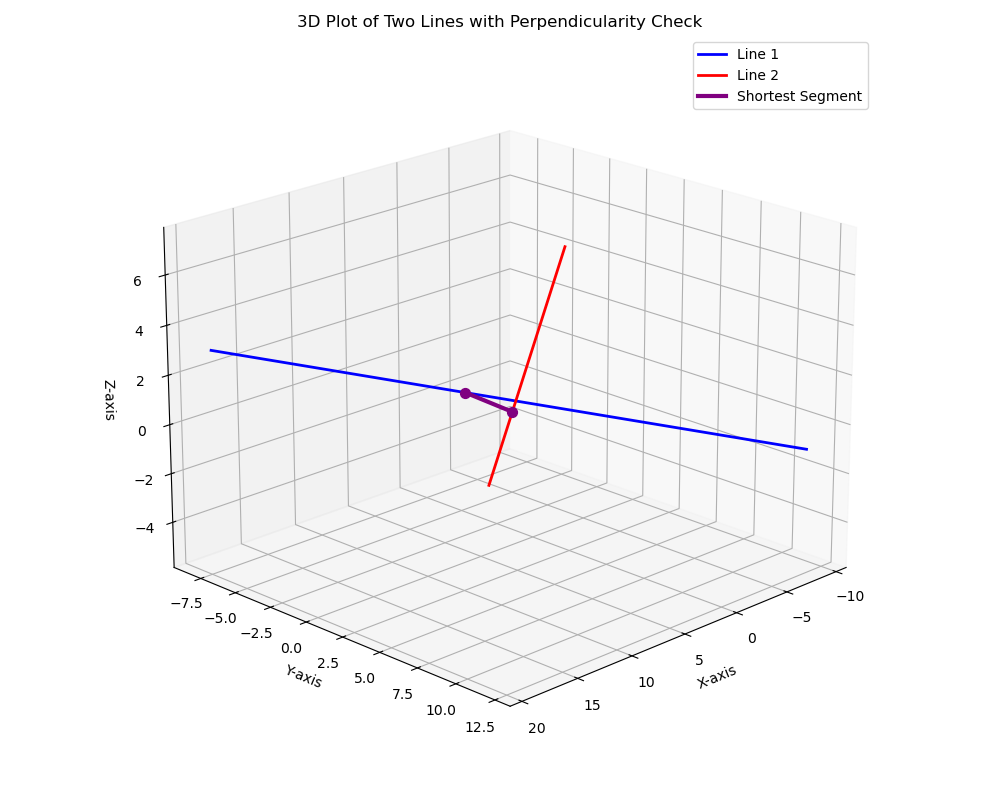
\includegraphics[width=0.9\columnwidth]{figs/fig.png}
    \caption{}
    \label{fig:placeholder2}
\end{figure}

\end{document}
